\section{Preliminary System Integration}

\subsection{Control System}
In October of 2010, I spent some time at the South Africa C-BASS beginning integration of various systems. The primary focus of this trip was to set the antenna up for control under the Owens Valley control system, so as to keep the systems identical. 

The trip was a success and the South African antenna is now usable with the OVRO control system. 

\subsection{Optical Pointing Model}
In order to test the reliability of the system, we also produced an optical pointing model. This involves a series of observations of stars (using a CCD camera and lens mounted to the antenna structure) at different positions across the sky. Since the positions of the stars are known, it is possible to produce a set of pointing errors defined by the direction in which the antenna is pointing. Various pointing effects ( mechanical misalignments, gravitational deformations etc.) are a function of the direction in which the antenna is pointing, and having a model for these offsets, allows the control system to compensate for them.

The optical pointing model used two nights worth of stellar observations and produced the results shown in Figure~\ref{fig:opticalPointing}. This shows a remarkably successful initial implementation.


\begin{figure}[ht]
 \centering
\subfloat[Crude Pointing model from tracking a single star across the sky. ]{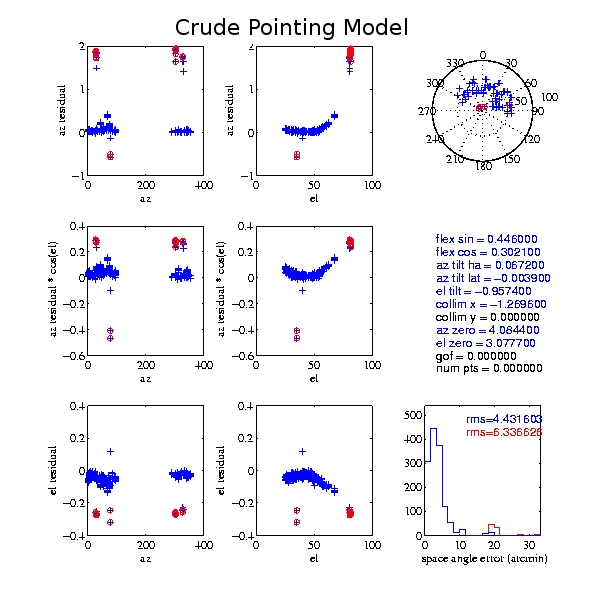
\includegraphics[width=0.45\textwidth]{images/control/CbassSouthNight2_1Labelled1.jpg}\label{fig:optPoint1}}
\hspace{0.1cm}
\subfloat[Refined pointing model using multiple evenly spaced sources. ]{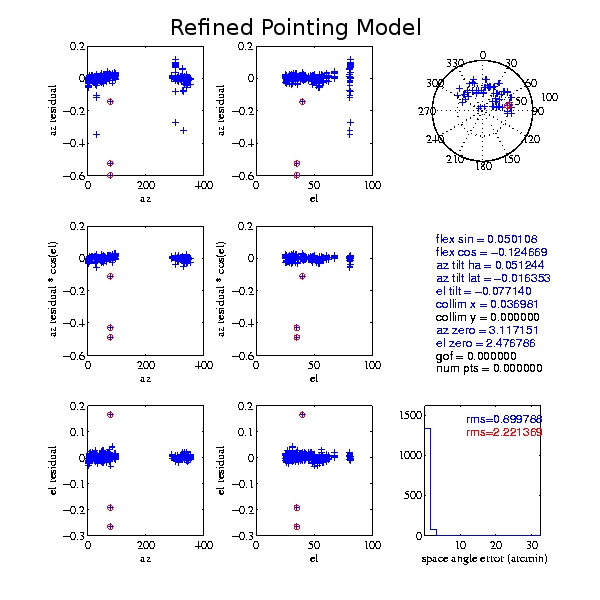
\includegraphics[width=0.45\textwidth]{images/control/CbassSouthNight2_7Labelled1.jpg}\label{fig:optPoint2}}\\
 % newdish_upgrade.jpg: 1280x728 pixel, 72dpi, 45.16x25.68 cm, bb=
 \caption{Improvement in the pointing model after one night's optical observations. Optical pointing improves from~$\approx$~4'~rms~to~\textless~1' rms. Red markers show large, probably spurious, recorded offsets and can either be included in the pointing error rms (red) or excluded (blue). Unfortunately we mistakenly used a Northern Hemisphere source list for Figure b resulting in the lack of sources in the Southern part of the sky. The pointing model used is described in \citeasnoun{Hill_M} }
 \label{fig:opticalPointing}
\end{figure}











\clearpage